%%%% ijcai21.tex

\typeout{IJCAI--21 Instructions for Authors}

% These are the instructions for authors for IJCAI-21.

\documentclass{article}
\pdfpagewidth=8.5in
\pdfpageheight=11in
% The file ijcai21.sty is NOT the same than previous years'
\usepackage{ijcai21}

% Use the postscript times font!
\usepackage{times}
\usepackage{soul}
\usepackage{url}
\usepackage{microtype}
\usepackage[hidelinks]{hyperref}
\usepackage[utf8]{inputenc}
\usepackage[small]{caption}
\usepackage{graphicx}
\usepackage{booktabs}
\usepackage{algorithm}
\usepackage{algorithmic}
\usepackage{courier}
\usepackage{color}
\usepackage{amsmath,amsfonts,amssymb,amsthm,amsopn}
\usepackage{epsfig}
\usepackage{booktabs}
\usepackage{array}
\usepackage{multicol}
\usepackage{threeparttable}
\usepackage{epstopdf}
\usepackage{listings}
\usepackage{multirow}
\usepackage{subfigure}
\usepackage{ragged2e}
\usepackage{xassoccnt}

\renewcommand{\algorithmicrequire}{ \textbf{Input:}}
\renewcommand{\algorithmicensure}{ \textbf{Output:}} 

\urlstyle{same}

% the following package is optional:
%\usepackage{latexsym}

% See https://www.overleaf.com/learn/latex/theorems_and_proofs
% for a nice explanation of how to define new theorems, but keep
% in mind that the amsthm package is already included in this
% template and that you must *not* alter the styling.
\newtheorem{example}{Example}
\newtheorem{theorem}{Theorem}

% Following comment is from ijcai97-submit.tex:
% The preparation of these files was supported by Schlumberger Palo Alto
% Research, AT\&T Bell Laboratories, and Morgan Kaufmann Publishers.
% Shirley Jowell, of Morgan Kaufmann Publishers, and Peter F.
% Patel-Schneider, of AT\&T Bell Laboratories collaborated on their
% preparation.

% These instructions can be modified and used in other conferences as long
% as credit to the authors and supporting agencies is retained, this notice
% is not changed, and further modification or reuse is not restricted.
% Neither Shirley Jowell nor Peter F. Patel-Schneider can be listed as
% contacts for providing assistance without their prior permission.

% To use for other conferences, change references to files and the
% conference appropriate and use other authors, contacts, publishers, and
% organizations.
% Also change the deadline and address for returning papers and the length and
% page charge instructions.
% Put where the files are available in the appropriate places.

%PDF Info Is REQUIRED.
\pdfinfo{
/TemplateVersion (IJCAI.2021.0)
}

\title{Grammatical error tagging and mask filling: a modulized approach to correct grammatical error}

% Single author syntax
% \author{
%     Zhi-Hua Zhou
%     \affiliations
%     Nanjing University
%     \emails
%     pcchair@ijcai-21.org\end{algorithmic}
% }

% Multiple author syntax (remove the single-author syntax above and the \iffalse ... \fi here)
% Check the ijcai21-multiauthor.tex file for detailed instructions
\iffalse
\author{
First Author$^1$
\and
Second Author$^2$\and
Third Author$^{2,3}$\And
Fourth Author$^4$
\affiliations
$^1$First Affiliation\\
$^2$Second Affiliation\\
$^3$Third Affiliation\\
$^4$Fourth Affiliation
\emails
\{first, second\}@example.com,
third@other.example.com,
fourth@example.com
}
\fi

\begin{document}

\maketitle

\begin{abstract}
We present a modulized architecture for Grammtical error correction (GEC). While recent works target to fine-tune a transformer-based pretrained model for this task, we devide the problem into two and construct correspendant modules, Grammatical Error Tagging and Mask Filling (GET-MF), for each of these two sub-problems. The GET module first predicts the edit tags for each token, the MF module suggests then the tokons regardign to the tags given by the GET module and effectuate the edits. The model achieves competitive accurancy on GEC task while improving the performance on certain types of errors like wrongly used collocations comparing to the state-of-the-art models for two reasons: On one hand, it shrinks the output dimension by optimizing the edit tag; on the other hand, it breaks the limit on the size of the editing space, which restricts vocabulary that can be effectuated for the corrections. 
\end{abstract}

\section{Introduction}

Protein$-$protein interactions (PPIs) are of central importance for the majority of biological functions, such as signal transduction, metabolic pathways, molecular dynamics, and protein networks\cite{Hoffmann.Krallinger.ea:2005}, for they serve as the most fundamental building blocks of the entire interacademic systems of any organisms. Collecting data on pairwise interaction relationships is essential for multiple purpose, including identification of modules with certain functionality\cite{Spirin.Mirny.03}, mapping diseases to dominated genes\cite{Ideker.Sharan.08}, and after all, understanding wholistic metabolic/genetic networks from a system biology perspective.

A lot of databases have been built to store protein and genetic interactions from major model organism species and are available in various standardized formats, such as MINT\cite{Zanzoni.Montecchi-Palazzi.ea:2002}, BIND\cite{Bader.ea:2003}, BIOGRID\cite{DBLP:journals/nar/StarkBRBBT06}, etc. Among those mainstream databases, the data largely rely on voluntary reports by scientists or researchers, besides, comprehensive curation efforts become indispensable for the sake of accuracy. However, the amount of biology-related literatures with respect to protein interactions grows explosively and thus make it either impossible or impractical to manually detect PPI information anymore.

Considering huge amount of PPI information with great wealth hidden in published papers, in recent years, numerous mining techniques have been proposed that aim to extract PPI information automatically from free text, especially machine learning, information retrieval, and natural language processing\cite{DBLP:journals/bib/WinnenburgWPDS08}.These approaches can be roughly categorized into three classes: co$-$occurrence, rule$-$based, and machine learning. 

Co$-$occurrence is the approach with most simplicity and naivete. Just as its name implies, this method intends to find out pairs of proteins that co-occur in the same context. The scope of "same context" ranges from phrase, sentence, paragraph to whole abstract, even document. The underlying assumption is that whenever two proteins are mentioned together by authors, chances are high that there is some kind of relationship between them. However, however, in-context closeness even semantic relation does not necessarily represent actual biological interaction. As a consequence, a large fraction of candidate pairs are mismatched inevitably, causing a high recall but low precision.

The second approach is rule-based extraction, in other words, pattern matching. There are many types of rules, most of them concern natural language processing (NLP). One way is to specify hand-crafted regular expressions before hand, which mostly lean on language usage preference. Besides, by using full or partial (shallow) parsing strategies, more information would be acquired, such as part-of-speech taggers, local dependencies between syntactic components, context-free grammar\cite{DBLP:journals/bioinformatics/TemkinG03}, and full sentence structure. Compared to co$-$occurrence, rule-based approach enjoy better precision but much lower recall. In addition, since the rules are usually derived from training data, that is to say, the improper choice of training data would be significantly lethal, therefore quality of extraction is invariably instable and may not applicable to other data.

The third and most commonly used approach use machine learning techniques, in this case, the task to extract protein$-$protein interactions turns out to be a binary classification problem. Each protein pairs are represented along with a set of features, which is associated with their context, then a well$-$defined classifier gives the answer whether the candidate protein pairs is classified to be qualified PPI. (TO BE FURTHER FILLED!!!)

In this paper, we introduce a general bootstrapping framework for Protein$-$protein interaction extraction from natural text.Our method differs from most of the previous works in three aspects:

(1)The extraction process is driven by only tiny fraction of training data, which are regarded as seed data. In each round, it would derive reliable patterns automatically from seed data, then extract more positive PPI pairs consequently, what's more, the seed data would be augmented by the newly extracted results with high confidence.

(2)multiple graph kernel. 

(3)various evaluation.




\section{Approach}
\label{sec:approach}
In this section, we first introduce the general framework of ChatMatch, which is modeled as
a sport tournament, then discuss some possible scoring functions that can be used by
the virtual judges in these competitions.

%Our whole evaluation framework consists of competition and scoring at three different levels. 
%The game level is at the bottom 
%and is played between two players. 
%Then comes the match level.
%To ensure the fairness of the game, 
%two games will be played between every two robots, 
%with each side starting a conversation.
%The result of two games determines the outcome of a match. 
%The tournament level is at the top
% and is composed of matches among different pairs of players. 

\subsection{Competition Protocol}
\label{sec:competition}
The competition takes place, from top to bottom, at tournament, match and
game levels.

\subsection*{Tournament Rules}
%\KZ{Give an overview of the how the tournament is run.}
We adopt a double round-robin 
sports tournament, where all bots participating in the competition 
converse directly with each other twice.
This is better than a knock-out system because it assesses a bot's ability to
deal with both strong and weak bots.
%For example, whether with weaker bots will induce them to make more mistakes or  how stronger bots will motivate their performance.
If we have $n$ chatbots players in our tournament, 
there will be $n\times (n-1) $ games in total.

\subsection*{Match Rules}
%\KZ{Talk about how the matches are administered. Just the procedure only.}
There are two chatbots competing in a single match. 
Each match consists of two games,
 started by a different bot. 
If we have $n$ bots in our tournaments, there 
will be ${n \choose 2}$ matches in total. 

\subsection*{Game Rules}
%\KZ{The procedure of the game. How each game is started and stopped.}
Each game is started by a player whose first utterance is provided by 
the system. The choice of the first utterance can be different 
depending on the domain of the bots and the ability we want to 
rank about the bots. For example, if we want to test 
the ability on movies, we can set a movie-related 
first utterance. 

During a game, there might be different ways to 
end the conversation. We can set a fixed number of exchanges 
or a terminating condition such as whether a bot makes a fatal error
or whether a certain score is reached.

\begin{table*}[th]
\centering
\scriptsize
\begin{tabular}{c|l|l}
%\hline
\toprule
\textbf{Dimension} & \textbf{Definition} &\textbf{Approach} \\ \midrule
Fluency  & Responses are fluent and natural.& Sentence perplexity. \\
Knowledge & Responses indicate the bot has the knowledge. & The number of times the bot expresses its ignorance to a question.\\
Proactivity & Responses actively proceed the conversation.&The number of times the bot raises a question. \\
Specificity & Responses are not generic.&The average of Distinct-1 and Distinct-2 \citep{li2015diversity}.\\
Diversity &Responses which are diverse and non-repetitive. &Repetition detection following the function in \algoref{algo:rep}. \\
Consistency &Responses do not contradict chat history. &Detect inconsistent questions following the function in \algoref{algo:inconsist}\\
Relevance & Responses are related to current context.& Ability to catch the relevant concept in chat history defined in \algoref{algo:bonus}. \\
\bottomrule
\end{tabular}
\caption{Seven evaluation dimensions.}
\label{tab:methods}
\end{table*}


\subsection{Scoring}
\label{sec:scoring}
\subsection*{Game-level Scoring}
%\KZ{Define a few functions: one to catch repeating, one to chat contradiction and one to catch long term memory.}

%Here we define the rules for recording points in one game between two bots. 
Inspired by \citet{finch2020towards}, 
we score each turn based on seven aspects of rules 
concerning \textit{consistency}, \textit{fluency}, \textit{knowledge}, \textit{specificity}, 
\textit{diversity}, \textit{relevance} and \textit{proactivity}. 
%As these seven metrics present a high level of 
%overlap among all distinct evaluation metrics used 
%during different process of human evaluation,
%we believe the combination of these seven distinct dimensions will be reliable. 
Finally, we sum up the scores for each bot for all the turns.
\tabref{tab:methods} documents the definition of these dimensions, which can all be scored
automatically.

%After finishing the calculation of the bonus and penalty scores for each turn, we obtain the scores of the two bots in a game with weighted sum according to \eqnref{eq:sum-up}

%\begin{equation}
%S(bot) = \sum_t - c\times C(t)  - r \times R(t) + b \times B(t)
%\label{eq:sum-up}
%\end{equation}
%$S$ denotes the total score gained by a bot for a game.
\begin{figure}[th]
        \centering
        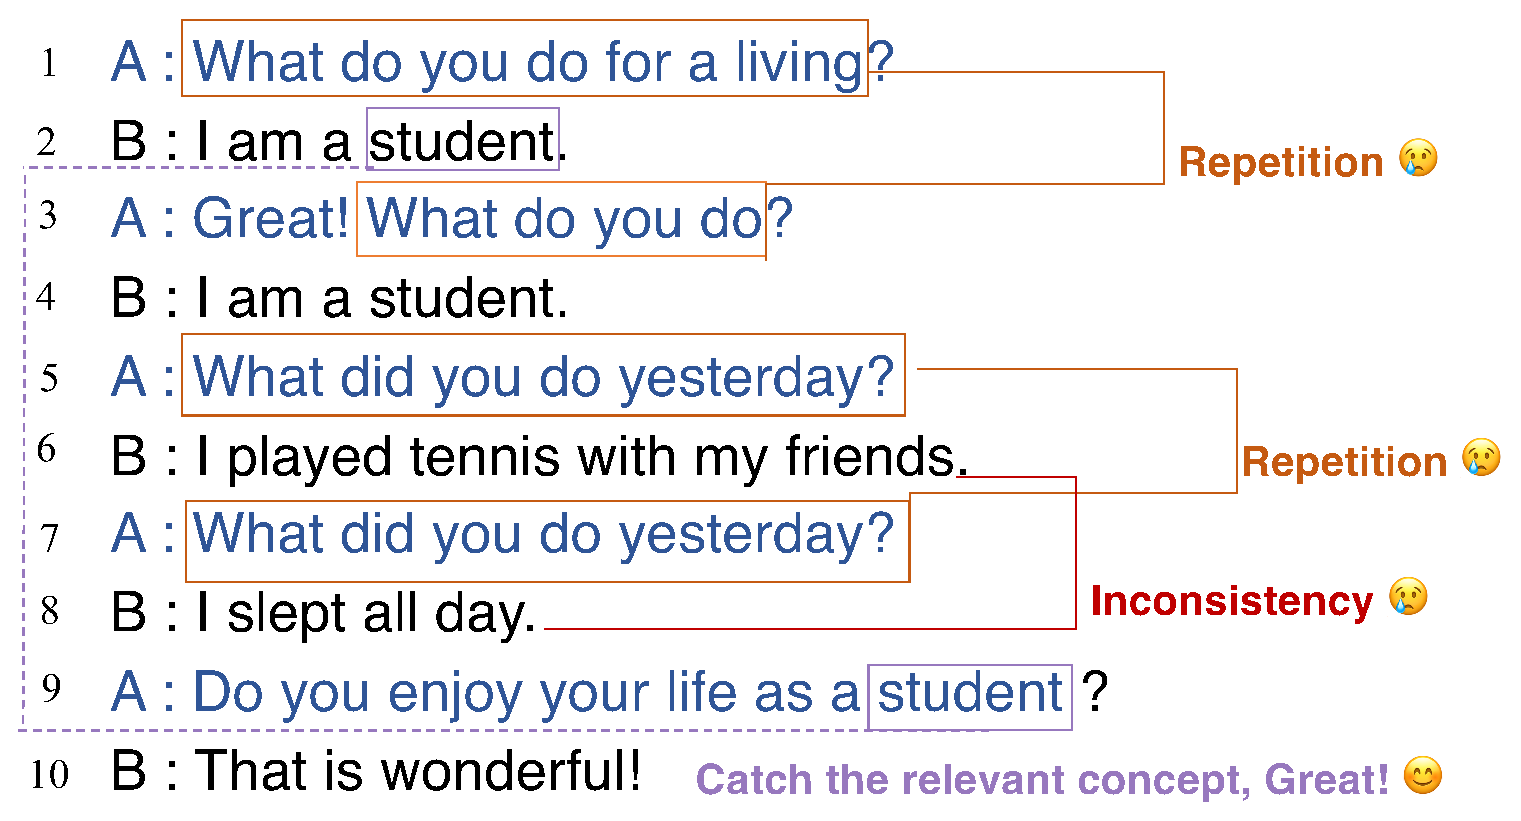
\includegraphics[width=0.95\columnwidth]{example2.eps}
        \caption{A chat snippet between two bots.}
        \label{fig:example}
\end{figure}

Fluency, Knowledge, Proactivity and Specificity are scored for each turn separately
and aggregated at the end of the conversation.
Detection for diversity, consistency and relevance are more involved and are explained
using \figref{fig:example}. 

As for diversity, at each turn $t$, we first check if there exists any repetitive question.  
We can easily find turn 3 and turn 7 repeated turn 1 and turn 5 
respectively. They will then be penalized one point for repetition. 
Repetition is not penalized if the previous turn is already 
marked as a repetitive question. For example, in \figref{fig:example}, 
although turn 4 is considered a repetition of turn 2,  
we are not going to penalize it as turn 3 is a repetitive question. 

The detection of inconsistency is always triggered after the detection of repeated questions. 
If the answers to the same questions are different, we will penalize the current turn, 
such as turn 8 in \figref{fig:example}.

We decide a repetition or an inconsistency by calculating the similarity of the two turns. 
We use a similarity function to complete the calculations, which we will 
discuss in \secref{sec:experiment}. The actual diversity and consistency scores
are the negation from the amount of repetition and inconsistency.

Relevance is assessed as a bonus to reward
a bot if it is able to memorize the important relevant concepts that have shown up 
before in the conversation. We sort the concepts that have shown up in 
chat history by their IDF scores. For example, in turn 9, $A$ 
mentions the concept word ``student'' presented by $B$ in turn 2. With this
turn, $A$ will win a bonus point.


The algorithms and notations for computing diviersty, consistency and relevance are included
in \tabref{tab:functions}, \algoref{algo:rep}, \algoref{algo:inconsist}, and \algoref{algo:bonus}. 

\begin{table}[th]
\centering
\small
\begin{tabular}{c|l}
%\hline
\toprule
\textbf{Notation} & \textbf{Description} \\ \midrule
$t$ & Current turn \\
$H(t)$  &  a list of history turns prior to $t$ \\
$Sim(x,y)$ & similarity between two turns $x$ and $y$ \\
$\sigma_r$ & Threshold for detecting repetition \\
$\sigma_c$ & Threshold for detecting consistency \\
$r$ & Weight for repetition \\
$c$ & Weight for inconsistency \\
$b$ & Weight for bonus \\
$d$ & Min distance between consecutive mentions \\
IDF list & List of lemma in chatlog sorted by IDF\\
$p$ & Percentage of important lemmas in IDF list\\
$R(t)$ &  Repetition penalty for turn $t$ \\
$C(t)$ &  Inconsistency penalty for turn $t$ \\ 
$B(t)$ &  Memory bonus for turn $t$ \\
$Rep(t)$ & A list of repeated turns for turn $t$ \\  
\bottomrule
\end{tabular}
\caption{
Functions and variables in algorithms.}
\label{tab:functions}
\end{table}

\begin{algorithm}[th]
\small
\caption{Scoring for Diversity}
\label{algo:rep}
\hspace*{0.02in} {\bf Input:}
 $t$, $H$, $Sim$, $\sigma_{r}$
; \hspace*{0.02in} {\bf Output: } 
 $R$;
\begin{algorithmic}[1]
\State //Starting to detect repetition
\For {$u$ in $H(t)$}
	\If {$Sim(t,u) \geq \sigma_{r}$}
		\State Add $u$ to $Rep(t)$
	\EndIf
\EndFor
    \If{$len(Rep(t))\geq 0$}
        \If{$t$ is a question and We can find a question in $Rep(t)$}
        \State $ R(t) \leftarrow  R(t) + 1$ 
        \Else
        \If {the previous turn of $t$ is not a repetitive question}
        \State $R(t)) \leftarrow R(t) + 1$ 
        \EndIf
        \EndIf
    \EndIf
\end{algorithmic}
\end{algorithm}


\begin{algorithm}[th]
\small
\caption{Scoring for Consistency}
\label{algo:inconsist}
\hspace*{0.02in} {\bf Input:}
$t$, $H$, $Sim$, $\sigma_{c}$
; \hspace*{0.02in} {\bf Output:  } 
 $C$;
\begin{algorithmic}[1]
\State // Inconsistency detection
 \If {previous turn of $p$ is a repetitive question} 
   \If{ the response $res$ to the question repeated by turn $p$ contradicts turn $i$ with $Sim(t, res) \leq \sigma_{c}$ }
    \State $C(t) \leftarrow C(t) + 1$
   \EndIf
  \EndIf
\end{algorithmic}
\end{algorithm}

\begin{algorithm}[th]
\small
\caption{Scoring for Relevance}
\label{algo:bonus}
\hspace*{0.02in} {\bf Input:}
$t$, $p$, $d$
; \hspace*{0.02in} {\bf Output:  } 
$B$;
\begin{algorithmic}[1]
\State // Assessing the ability of catching relevant concepts\\
$B(t) \leftarrow 0$
\For {all tokens $tk$ in current turn $t$}
 \If {$t$ - previous occurrence turn of $tk > d$ and $tk$ in the top $p\%$ of the IDF list of all tokens in the dialogue} 
   \State $B(t) \leftarrow 1$
  \EndIf
 \EndFor
\end{algorithmic}
\end{algorithm}

At the end of each game, each bot gets seven scores, one for each dimension.  
After pairwise comparison on individual dimension, a bot gains one point for win and zero point for a tie or lose.
The final score of each bot is determined by the sum of their individual scores.
%\KZ{Are these scores positive or negative? Comparable between bots?}

\subsubsection*{Match-level Scoring}
%\KZ{Use an equation to compute the final scores?}
One match which consists of two games, each started with a different bot, 
decides winning or losing between two bots.
For match-level scoring, we mimic the scoring rules of soccer tournament. 
For each match, $W$ points for the winner,  
$T$ points for a tie and 
$L$ points for the loser.
The value of $W$, $T$ and $L$ will be discussed in \secref{sec:ablation}. 

%\KZ{At the match level, we need to consider different starting context for the bots? I think we should present a few options for the reader and say that we are limited to these.}

\subsubsection*{Tournament-level Scoring}
%\KZ{Use an equation to compute the final scores?}
We count the points by simply summing up their scores gained in every match. Currently, several bots with the same final rank are tolerated. For future study, it's possible to mimic more detailed rules presented in sports match such as determine their ranking based on their win-loss relationship in the match between them.  
If they are still tied, we could propose an “overtime” for these two bots, one human judge may observe their performance and then make the decision of the game.

\section{Experimental Results}
% \KZ{Put a preamble here... In general, don't use the word ``prove'' unless you
% have mathematical proof. Experiments can only ``show'' or 
% ``demonstrate'' things, not prove things.}

In this section, we first introduce the experimental setup, including dataset, baselines, evaluation metrics, and implementation details. Then, we show the results and compared with five unsupervised baselines and six supervised+domain-adapted baselines in \secref{sec:result}. Finally, we analyze the result from four aspects: the effects of different datasets, ablation study, case study, 
and human evaluation.

\subsection{Datasets}
We evaluate our framework on four different datasets, namely Quora, WikiAnswers, MSCOCO, and Twitter. Following \citet{liu2019unsupervised}, we randomly choose 20K parallel paraphrase pairs as the test set and 3K parallel paraphrase pairs as the validation set for Quora, WikiAnswers, and MSCOCO. 

We randomly sample the remaining parallel paraphrases pairs and pick one sentence from each pair to construct the non-parallel training data.
The number of selected sentences is the same as the work by \citet{liu2019unsupervised}, which is 400K for Quora, 500K for WikiAnswers, 320K for MSCOCO and 110K for Twitter.

\paragraph{Quora. } Quora\footnote{You can find the dataset at \url{https://data.quora.com/First-Quora-Dataset-Release-Question-Pairs}} dataset is released by Quora in
January 2017. It contains 400K pairs of questions with manual annotation about whether questions in each pair are duplicates of each other. Through these annotations, there are 140K pairs marked as paraphrases and 320K pairs masked as non-paraphrases. 

\paragraph{WikiAnswers. } WikiAnswers \citep{fader2013paraphrase} dataset contains 2.3M pairs of question paraphrases extracted from the WikiAnswers website. The dataset is collected automatically without manual annotation.

\paragraph{MSCOCO. } MSCOCO \citep{lin2014microsoft} contains human-annotated captions for 120K images. Each image contains five captions considered as paraphrases of each other, we take four pairs from each image and get 500K parallel pairs.

\paragraph{Twitter. } Twitter \citep{lan2017continuously} is a paraphrase detection dataset, containing 110K pairs of potential paraphrases and 60K manually annotated paraphrases. There are only 600 sentences marked as paraphrases in the test set, and we take them all for testing.

\paragraph{Training on Common-Domain Data} \label{sec:indomain}
When there is no sufficient target-domain non-parallel data, or when we cannot use any data from the target-domain to train the set2seq model, it is hard to train unsupervised models or fine-tune supervised models in the target-domain. Our solution is to train the set2seq model with a big common-domain dataset and apply it to the target-domain. We name the model ``set2seq-common''. We test the performance of our framework with set2seq-common on four datasets to show the generality of our framework. Further, we apply set2seq-common in \secref{sec:app} for data augmentation since we cannot train the set2seq model with the translation data to be augmented.

\subsection{Baselines and Evaluation Metrics}
We compare our framework with five unsupervised methods and six supervised methods with domain adaptation. We re-produce ParaNMT and ParaBank with our translation models, and take the results from \citet{liu2019unsupervised} for other baselines. For a fair comparison, we keep their scripts for data pre-processing and evaluation. On the Quora dataset, we even use the same train-test split as UPSA.\footnote{The pre-processing script, evaluation script, train-test split and results of UPSA can be found at \url{https://github.com/anonymity-person/UPSA}}
% For human evaluation, we use the open source code and data provided by UPSA and CGMH\footnote{\url{https://github.com/NingMiao/CGMH}}, and take the same VAE tool used by 
% \citet{liu2019unsupervised} to generate some paraphrases on the Quora dataset.

\paragraph{Unsupervised methods. } The current state-of-the-art unsupervised method is Unsupervised Paraphrasing by Simulated Annealing (UPSA), proposed by \citet{liu2019unsupervised}, which is also our main target of comparison. Other unsupervised methods include CGMH from \citet{miao2019cgmh}, ParaNMT from \citet{wieting2017paranmt}, ParaBank(-$3^{rd}$ IDF) from \citet{hu2019parabank}, and VAE from \citet{kingma2013auto}. Note that ParaNMT used back-translation to generate paraphrases, so it can be viewed as ``back-translation only''.

\paragraph{Supervised methods with domain adaptation. } Decomposable Neural Paraphrase Generation (DNPG) \citep{li2019decomposable} is the current state-of-the-art method for supervised paraphrase generation.
% \citet{li2019decomposable} raised the issue of domain adaptation in his paper and demonstrated that DNPG also performed best with domain adaptation, so we mainly compare our framework with DNPG. 
Other baselines are shallow fusion from \citet{gulcehre2015using}, Multi-Task Learning (MTL) from \citet{domhan2017using}, Pointer-generator from \citet{see2017get}, Transformer \citep{vaswani2017attention} with copy mechanism, and MTL with copy mechanism. 

\paragraph{Evaluation metrics. } For the fairness of comparison, 
we take the same evaluation metrics as in UPSA and 
DNPG, which are iBLEU \citep{sun2012joint}, BLEU \citep{papineni2002bleu} and ROUGE \citep{lin2004rouge} scores. 
BLEU and ROUGE scores are common evaluation metrics for NLP tasks while 
iBLEU is especially designed for paraphrase generation tasks. 
It penalizes the similarity between paraphrase and the original sentence. 
Suppose the input sentence is $src$, the output paraphrase is $out$, 
and the ground truth paraphrase is $trg$, we calculate iBLEU as follows:
\begin{multline}
\text{iBLEU} = \alpha \cdot \text{BLEU}(out, trg) - \\
(1-\alpha) \cdot \text{BLEU}(out, src)
\end{multline}
BLEU and ROUGE only consider the accuracy but ignore the 
diversity of generated paraphrases, while iBLEU considers both. 
So we use iBLEU as our main evaluation metric.
We set $\alpha=0.9$, same as other baselines.

\begin{table*}[ht]
\small
\centering
\begin{tabular}{p{2cm}p{3.4cm}p{0.8cm}<{\centering}p{0.8cm}<{\centering}p{0.8cm}<{\centering}p{0.8cm}<{\centering}p{0.8cm}<{\centering}p{0.8cm}<{\centering}p{0.8cm}<{\centering}p{0.8cm}<{\centering}}
\hline
\\ [-1.7ex]
& & \multicolumn{4}{c}{\textbf{Quora}} & \multicolumn{4}{c}{\textbf{WikiAnswers}} \\
\\ [-1.7ex]
\cline{3-6} \cline{7-10} 
\\ [-1.8ex]
 &Model&iBLEU&BLEU&R-1&R-2&iBLEU&BLEU&R-1&R-2\\
\\ [-1.8ex]
\hline
\\ [-1.8ex]
Supervised & DNPG (SOTA) & 
18.01 & 25.03 & 63.73 & 37.75 & 34.15 & 41.64 & 57.32 & 25.88 \\
\\ [-1.8ex]
\hline
\\ [-1.8ex]
\multirow{6}{3cm}{Supervised + \\Domain-Adapted}
& Pointer-generator & 
5.04 & 6.96 & 41.89 & 12.77 & 21.87 & 27.94 & 53.99 & 20.85 \\
& Transformer+Copy &
6.17 & 8.15 & 44.89 & 14.79 & 23.25 & 29.22 & 53.33 & 21.02 \\
& Shallow fusion &
6.04 & 7.95 & 44.87 & 14.79 & 22.57 & 29.76 & 53.54 & 20.68 \\
& MTL &
4.90 & 6.37 & 37.64 & 11.83 & 18.34 & 23.65 & 48.19 & 17.53 \\
& MTL+Copy &
7.22 & 9.83 & 47.08 & 19.03 & 21.87 & 30.78 & 54.10 & 21.08 \\
& DNPG &
10.39& 16.98& 56.01 & 28.61 & \underline{25.60} & \underline{35.12} & \underline{56.17} & \underline{23.65} \\
\\ [-1.8ex]
\hline
\\ [-1.8ex]
\multirow{8}{3cm}{Unsupervised}
& VAE & 
8.16 & 13.96 & 44.55 & 22.64 & 17.92 & 24.13 & 31.87 & 12.08 \\
& ParaNMT\scriptsize{(back-translation)} & 
10.69& 15.75 & 52.28 & 25.12 & 14.94 & 20.01 & 30.55 & 10.23 \\
& ParaBank & 
9.92 & 14.71 & 50.03 & 23.80 & 13.14 & 17.56 & 28.97 & 9.34 \\
& CGMH & 
9.94 & 15.73 & 48.73 & 26.12 & 20.05 & 26.45 & 43.31 & 16.53 \\
& UPSA & 
\underline{12.02}& \underline{18.18} & \underline{56.51} & \underline{30.69} & 24.84 & 32.39 & 54.12 & 21.45 \\
\\ [-1.8ex]
\cline{2-10}
\\ [-1.8ex]
& set2seq \scriptsize{(ours)} & 
13.54 & 20.85 & 58.27 & 32.59 & 25.98 & 33.41 & 55.95 & 23.08 \\
& set2seq-common+BT \scriptsize{(ours)} & 
12.60 & 18.85 & 57.13 & 31.19 & 25.04 & 33.43 & 55.81 & 23.12 \\
& set2seq+BT \scriptsize{(ours)} & 
\textbf{14.66} & \textbf{22.53} & \textbf{59.98} & \textbf{34.09} & \textbf{28.27} & \textbf{37.42} & \textbf{56.71} & \textbf{24.94} \\
\\ [-1.8ex]
\hline
\\ [-1.5ex]
& & \multicolumn{4}{c}{\textbf{MSCOCO}} & \multicolumn{4}{c}{\textbf{Twitter}} \\
\\ [-1.7ex]
\cline{3-6} \cline{7-10} 
\\ [-1.8ex]
 &Model&iBLEU&BLEU&Rouge1&Rouge2&iBLEU&BLEU&Rouge1&Rouge2\\
\\ [-1.8ex]
\hline
\\ [-1.8ex]
\multirow{8}{3cm}{Unsupervised}
& VAE & 
 7.48 & 11.09 & 31.78 &  8.66 &  2.92 &  3.46 & 15.13 &  3.40 \\
& ParaNMT\scriptsize{(back-translation)} & 
 7.39 & 10.71 & 30.74 &  8.68 &  \underline{7.57} & \underline{10.79} & \underline{35.38} & \underline{14.74} \\
& ParaBank & 
 6.45 &  9.48 & 29.22 &  8.35 &  6.50 &  9.71 & 34.56 & 13.92 \\
& CGMH & 
 7.84 & 11.45 & 32.19 &  8.67 &  4.18 &  5.32 & 19.96 &  5.44 \\
& UPSA & 
 \underline{9.26} & \underline{14.16} & \underline{37.18} & \underline{11.21} &  4.93 &  6.87 & 28.34 &  8.53 \\
\\ [-1.8ex]
\cline{2-10}
\\ [-1.8ex]
& set2seq \scriptsize{(ours)} & 
\textbf{11.54} & 17.61 & 39.87 & 13.67 & 5.72 & 7.48 & 31.65 & 10.89 \\
& set2seq-common+BT \scriptsize{(ours)} & 
 9.07 & 13.44 & 35.90 & 11.05 &  9.73 & \textbf{14.30} & \textbf{39.23} & \textbf{18.82} \\
& set2seq+BT \scriptsize{(ours)} & 
11.39 & \textbf{17.93} & \textbf{40.28} & \textbf{14.04} & \textbf{9.95} & 13.97 & 38.96 & 18.32 \\
\\ [-1.8ex]
\hline
\end{tabular}
\caption{\label{tab:result}
Evaluation results on Quora, WikiAnswers, MSCOCO and Twitter. The comparison 
with supervised + domain adapted methods is only on Quora and WikiAnswers 
because results of current state-of-the-art 
method~\citep{li2019decomposable} are only available on these two datasets.
}
\end{table*}

\subsection{Implementation and Training Details} \label{sec:exset}
To be consistent with the pre-processing of UPSA and DNPG, we convert the input words into lower-case and truncate all sentences to up to 20 words. 
For the convenience of hybrid decoding, 
we learn a shared byte-pair encoding (BPE, \citet{sennrich2016edinburgh}) 
with size 50k from the training data for translation models, 
and use a 30K vocabulary for all models. Same as UPSA and DNPG, all baselines include all words that appear in the training set into the vocabulary for a fair comparison. For the hyper-parameter $\lambda$ mentioned in 
\secref{sec:joint}, we set it to 0.5 for all datasets(chosen from $\{0.1, 0.2, \cdots, 1, 2, 3\}$).

For the translation models in back-translation, we train them with the WMT17\footnote{\url{http://statmt.org/wmt17/translation-task.html}} zh-en dataset \citep{ziemski2016united}. We train them with a standard transformer for 3 days on two GTX-2080 GPUs. We reuse these translation models for ParaNMT and ParaBank. For the set2seq-common model mentioned in \secref{sec:indomain}, we use the news-crawl-2016 English monolingual data from WMT17 and train 1.5 days with a standard transformer. For the domain-specific set2seq models, we use a 2-layer transformer with 300 embedding size, 256 units, 1024 feed-forward dimensions for all layers to train them. The training lasts 3 hours on a single GTX-2080 GPU. Set2seq is a lightweight model with 31M parameters, 3.7M parameters for multi-head attention layers, only one-third of a standard transformer.

To calculate iBLEU and BLEU, four references are used for MSCOCO, five for WikiAnswers, and one for other datasets. For some test cases, WikiAnswers does not have 5 references, so we evaluate them on reduced references. 
For ROUGE scores, we take the average of all references.

\subsection{Results} \label{sec:result}

Table~\ref{tab:result} presents our experimental results. We mark the previous highest scores by underlining them and mark the present highest scores with the bold font.
The supervised method (DNPG (SOTA)) here is only for reference.

We compare three different models with the previous methods, 
namely set2seq, set2seq-common+BT, and set2seq+BT, where BT stands for 
back-translation. We show the set2seq alone here to demonstrate that
useful information comes not only from translation, as the
set2seq model alone can already outperform almost all competitors. 

Our framework outperforms all existing unsupervised methods and supervised methods with domain adaptation. The results from our framework are even close to the state-of-the-art supervised model DNPG. 

\subsection{Analysis} \label{sec:analysis}
\paragraph{Datasets. } Due to the domain-specific differences between four datasets, it is understandable that scores on all metrics vary a lot across different datasets. Sentences in Quora and WikiAnswers are of the best quality.
% , they are in appropriate lengths and have high correlations between paraphrases in the same pair. 
Experiments on these two datasets are the most persuasive and representative.

Paraphrases from MSCOCO are descriptions of images, the set2seq model fits this dataset quite well since the process of generating paraphrases are similar: 
one extends information from a static picture; 
the other extends from a word set. 
The set2seq-common model cannot learn the in-domain properties of MSCOCO, 
so it does relatively poorly here as opposed to its performance 
in other datasets. 

Lack of training data for Twitter leads to insufficient training of most models. Models containing back-translation perform extraordinary well since they have adequate information. Besides, set2seq-common+BT achieves an excellent result, which shows the advantages of the set2seq-common model compared with the set2seq model trained with insufficient in-domain data.

\paragraph{Ablation Study. }

Table~\ref{tab:ablation} shows the result of the ablation study on the Quora dataset, where $\text{BLEU}_{ref}$ is the BLEU between reference and output, the higher the better and $\text{BLEU}_{src}$ is the BLEU between source sentence and output, the lower the better. 

We demonstrate that removing stopwords outperforms retaining high-IDF words. For high-IDF words, we keep top $k\%$ high-IDF words in the original sentence. For the value of $k$, we set $k=50$, which is the best among $[30, 40, 50, 60, 70]$. We also tried TextRank \citep{mihalcea2004textrank} to score words and get similar results with IDF scores. 

Removing random replacement and adding position encoding can both lead to 
a high BLEU between source sentences and output paraphrases, 
which substantially reduces the diversity of generated sentences. 
% \KZ{Consider dropping this: 
% We try to augment the NMT training data with these two methods in 
% section~\ref{sec:app}, but fail to get any improvement. 
% Since we do not mainly conduct NMT experiments, we only propose an observed phenomenon here, more detailed experiments can be done in future works.}

\begin{table}
\small
\centering
\begin{tabular}{lp{0.8cm}<{\centering}p{1cm}<{\centering}p{1cm}<{\centering}}
\hline 
\\ [-1.8ex]
\textbf{Model Variants} & iBLEU & $\text{BLEU}_{ref}$ & $\text{BLEU}_{src}$ \\
\\ [-1.8ex]
\hline
\\ [-1.8ex]
set2seq+BT & \textbf{14.66} & 22.53 & \textbf{56.17} \\
\\ [-1.8ex]
\hline
\\ [-1.8ex]
\multicolumn{1}{m{3cm}}{$\ominus$ excluding stopwords \par $\oplus$ retaining high-IDF} & 13.46 & 22.15 & 64.75 \\
\\ [-1.8ex]
\hline
\\ [-1.8ex]
\multicolumn{1}{m{3cm}} {$\ominus$ random replacement} & 13.78 & \textbf{23.92} & 77.47 \\
\\ [-1.8ex]
\hline
\\ [-1.8ex]
\multicolumn{1}{m{3cm}}{$\oplus$ position encoding} & 14.07 & 23.26 & 68.60 \\
\\ [-1.8ex]
\hline
\end{tabular}
\caption{\label{tab:ablation} Ablation Study on Quora.}
\end{table}

\paragraph{Case Study. } Table~\ref{tab:case} shows the examples of generated paraphrases through different strategies.

Two kinds of information are easily lost in set2seq: 
one is the information in stopwords; the other is the information in the 
sequential expression. 
In the first example, set2seq model loses the word ``When'' 
when generating paraphrase from the word set. 
In the second example, set2seq model mistakes the relationship between the 
the universe and the black hole since it cannot obtain any sequential information. 

For back-translation, the correct paraphrase sometimes cannot be 
generated due to the limited capacity of the translation models, 
``seed funding'' should be a fixed phrase in Example 3, 
but back-translation cannot recognize it.

% For seq2seq+BT, the generated sentences are too close to the 
% original sentences by the order of the words. 
% Our goal is to generate sentence level paraphrases, 
% but seq2seq model limits the sequential expression.

\begin{table}
\small
\centering
\begin{tabular}{lp{4.6cm}}
\hline 
\\ [-1.8ex]
\textbf{Example 1} & \\
\\ [-1.8ex]
\hline
\\ [-1.8ex]
Input & when will be end of world ? \\
Word Set & (stop, earth, ?) \\
BT & when is the end of the world ? \\
set2seq & will the world end ? \\
% seq2seq+BT & what is the end of the world ? \\
set2seq+BT & when will the world end ? \\
\\ [-1.8ex]
\hline
\\ [-1.8ex]
\textbf{Example 2} & \\
\\ [-1.8ex]
\hline
\\ [-1.8ex]
Input & could this universe be inside a black hole ? \\
Word Set & (universe, in, dark, cave, ?) \\
BT & can universe be a black hole ? \\
set2seq & is there a black hole in the universe ? \\
% seq2seq+BT & could the universe be in a black hole ? \\
set2seq+BT & is the universe in a black hole ? \\
\\ [-1.8ex]
\hline
\\ [-1.8ex]
\textbf{Example 3} & \\
\\ [-1.8ex]
\hline
\\ [-1.8ex]
Input & do product ideas get seed fundings ? \\
Word Set & (produce, mind, incur, germ, financing, ?) \\
BT & does the product concept receive seed money ? \\
set2seq & where can i get funding for my product idea ? \\
% seq2seq+BT & do product ideas get seed funding ? \\
set2seq+BT & how do i receive seed funding for my product idea ? \\
\\ [-1.8ex]
\hline
\end{tabular}
\caption{\label{tab:case} Case Study }
\end{table}
% \KZ{The fonts in Table 4 too small.}
\begin{table}[th]
\small
\centering
\begin{tabular}{lcc}
\hline 
\\ [-1.8ex]
\textbf{Method} & Accuracy & Fluency \\
\\ [-1.8ex]
\hline
\\ [-1.8ex]
VAE & 2.48 & 3.44 \\
CGMH & 2.97 & 3.67 \\
UPSA & 3.52 & 3.69 \\
back-translation & 3.50 & \textbf{4.52}\\
set2seq+BT\scriptsize{(ours)} & \textbf{3.98} & 4.43 \\
\\ [-1.8ex]
\hline
\end{tabular}
\caption{\label{tab:human} Results for Human Evaluation. }
\end{table}

\paragraph{Human Evaluation.}
We choose 100 sentences from Quora and ask 3 human annotators to score the result from 1 to 5 from the perspective of both fluency and accuracy without telling them the result is generated by which method, the higher score indicates the better quality of the generated paraphrases. From the perspective of fluency, we judge whether paraphrase conforms to grammar and common sense. From the perspective of accuracy, we judge whether paraphrase has the same meaning as the original sentence but expressed differently.

% For UPSA and CGMH\footnote{CGMH: \url{https://github.com/NingMiao/CGMH}}, they provided open-source code and data, and for VAE, we use the code from SentenceVAE\footnote{\url{https://github.com/timbmg/Sentence-VAE}}. 

We can see that word/phrase based methods have bad performances on fluency since their Language Model is trained on a small dataset. Paraphrases generated by back-translation are not very accurate since they are not trained by in-domain data. From the perspective of both fluency and accuracy, our method performs 
the overall best.
% All annotators are asked to 
% consider the result from both accuracy and diversity. We give a reference for scoring:
% \begin{itemize}
% \item[\textbf{1.}] The meaning is totally different.
% \item[\textbf{2.}] Exactly the same sentence.
% \item[\textbf{3.}] The meaning is slightly different.
% \item[\textbf{4.}] Express the same meaning in a slightly different expression.
% \item[\textbf{5.}] Express the same meaning in a totally different expression.
% \end{itemize}
% Table~\ref{tab:human} shows the average rating of 
% all annotators on all sentences. 
% Our framework performs the best among different baselines. 

% \section{Applications}
\label{sec:application}
AliCoCo has already supported a series of downstream applications in Alibaba's ecosystem, especially in search and recommendation, two killer applications in e-commerce.
In this section, we introduce some cases we already succeed, those we are attempting now, and some other we would like to try in the future.

\subsection{E-commerce Search}

\subsubsection{Search relevance}
% 直接用isa关系,搜索相关性1个点的auc, 线上bad case下降4%

Relevance is the core problem of a search engine, and one of the main challenges is the vocabulary gap between user queries and documents. 
This problem is more severe in e-commerce since language in item titles is more professional. 
Semantic matching is a key technique to bridge the gap in between to improve relevance.
IsA relations is important in semantic matching. 
For example, if a user search for a ``top'', search engine may classify those items whose title only contains ``jacket'' but without ``top'' as irrelevance.
Once we have the prior knowledge that ``jacket is a kind of top'', 
this case can be successfully solved.
Comparing to a former category taxonomy, which only has 15k different category words and 10k isA relations,
AliCoCo containing 10 times categories words and isA relations.
Offline experiments show that our data improves the performance of the semantic matching model by $1\%$ on AUC, 
and online tests show that the number of relevance bad cases is dropped by $4\%$, meaning user satisfaction is improved.

\subsubsection{Semantic search \& question answering}
% semantic search,本体的理解
As shown in \figref{fig:cloud}(a),
semantic search empowered by AliCoCo is ongoing at the time of writing. 
Similar to searching ``China'' on Google and then getting a knowledge card on the page with almost every important information of China, 
we are now designing a more structured way to display the knowledge of ``Tools you need for baking'' once a customer searching for ``baking''.
On the other hand, this application requires a high accuracy and recall of relations, which are still sparse in the current stage of AliCoCo.
Question answering is a way of demonstrating real intelligence of a search engine. 
Customers are used to keyword based search for years in e-commerce.
However, at some point we may want to ask an e-commerce search engine ``What should I prepare for hosting next week's barbecue?''. 
We believe AliCoCo is able to provide ample imagination towards this goal with continuous efforts to integrate more knowledge especially concerning common sense.

\subsection{E-commerce Recommendation}

\subsubsection{Cognitive recommendation}
% 云主题,0-1全新的产品,用户体感提升,推荐创新
As we introduce in \secref{sec:intro},
a natural application of e-commerce concepts is directly recommending them to users together with 
its associated items.
In the snapshot shown in \figref{fig:cloud}(b), concept ``Tools for Baking'' is displayed as a card, with the picture of a representative item.
Once users click on this card, 
it jumps to a page full of related items such as egg scrambler and strainer.
We perform thorough offline and online experiments in a previous work
\cite{luo2019conceptualize}.
It has already gone into production for more than 1 year with high click-through rate and satisfied GMV (Gross Merchandise Value).
According to a survey conducted by online users, 
this new form of recommendation brings more novelty and further improve user satisfaction. 
This application is totally based on the complete functionality of AliCoCo, which demonstrates its great value and potential. 



\subsubsection{Recommendation reason}

% 推荐理由,正在尝试
The advantages of e-commerce concepts include its clarity and brevity, which make them perfect recommendation reasons to display when recommending items to customers.
This idea is currently experimented at the time of writing.



\section{Related Work}
This section surveys previous works on question generation and tree encoding
respectively.

Text question generation has attracted the attention 
after the work of ~\citeauthor{du2017learning}~\shortcite{du2017learning}, who uses deep seq2seq model 
to generate questions from a raw text paragraph. 
Before that, text question generation relied heavily on hand-craft 
question patterns~\cite{HeilmanS10,LabutovBV15,MostowC09} which is time and 
labor consuming. 

However, this pure seq2seq model is not focused and 
has no control over part in the paragraph to generate question. 
~\citeauthor{zhou2017neural}~\shortcite{zhou2017neural} proposed to encode 
key phrase information using binary indicators to generate 
key-aware questions and they assumes the answer to be key phrase. 
Considering key phrase (answer) is unavailable in reality, 
~\citeauthor{SubramanianWYT17}~\shortcite{SubramanianWYT17} applied 
a two-stage approach. First, key phrases are extracted by 
pointer network~\cite{ptrnet}. Second, 
key phrases are encoded in the same way as 
Zhou et al. With the intuition that questions could be asked in many ways, 
~\citeauthor{Yao2018vae}~\shortcite{Yao2018vae} used conditional-VAE to 
increase the diversity of questions. More recently, models with 
auxiliary feature information~\cite{HarrisonW18} helped improve 
the question quality. Structure question generation aims at 
converting structured data such as triples in knowledge graph to questions. 
~\citeauthor{SerbanGGACCB16}~\shortcite{SerbanGGACCB16} proposed a model to generate factoid questions from knowledge base triples.  None of the above work
considered using parse tree structures to aid question generation process,
which is the focus of this paper.

Sequential RNN model takes sentence as a sequence of words, 
ignoring the syntactic information. In order to utilize
such syntactic information with sequential information, 
~\citeauthor{tai2015improved}~\shortcite{tai2015improved} proposed Tree-LSTM to 
encode the binary parse tree recursively in a bottom-up fashion to 
classify sentiment. In text generation task, 
\citeauthor{eriguchi2016tree}~\shortcite{eriguchi2016tree} 
proposed a tree-to-sequence model with attention mechanism to do 
machine translation and 
~\citeauthor{liang2018automatic}~\shortcite{liang2018automatic} proposed a 
tree-to-sequence model which could handle arbitrary trees, 
to do code comment generation. Our work is inspired by these previous
attempts and we are first to adapt structure encoded neural models to
textual question generations.
\section{Conclusion}
We implement a novel sequence-based dependency parsing
framework which takes advantage of high order features 
in parsing history. 
%We can also adapt beam search to this framework so as to
%relax the strictly greedy nature. Vine pruning\cite{rush2012vine} could
%be incorporated to speed up the parsing.
More importantly, we discovered that the parsing accuracy is very sensitive to
the quality of parsing sequence. Future work can be focused on
developing better sequence predictors that outperform Malt action classifier.
Furthermore, we use two sets of features for sequence predictor and
head mapper right now. A unified set of features between these two components
are worth exploring.
%Besides, better sequence predicting method and unified feature
%representation of two components are worth exploring.
%
%Though we currently get a not bad result,
%the sequence predictor still needs more exploration.
%According to our experiment, slightly changes
%on the sequence can lead to a fatal decline on accuracy. Ensuring the match degree of training sequence and testing
%sequence demands a high quality of sequence predictor.
%
%Further, the features in our current implementation are not expanded and well tuned yet  and we are free to define high order features to make use of parsing history. Our framework is flexible to merge other technics to enhance the performance. Introducing beam could make up for our greedy decoder and improve our accuracy. Vine pruning\cite{rush2012vine} could speed up parsing process. Besides, better sequence predicting method and unified feature representation of two components are worth exploring.


%% The file named.bst is a bibliography style file for BibTeX 0.99c
\bibliographystyle{named}
\bibliography{paper.bib}

\end{document}

